% -*- root: ../main.tex -*-
\chapter{Introduction\label{chap:introduction}}

\paragraph{Abstract}

In this chapter we will introduce this bachelor thesis.
%
We will cover the motivation that led the development of this \thisworkm and which objectives we pursue.

We will discuss its scope, the document structure and finally we will introduce the preliminaries, describing some concepts needed during the whole bachelor thesis. 

\section{Motivation}

\label{Motivation}
Last May $\text{2}^{\text{nd}}$ a Japanese satellite was lost in space. This satellite cost \$248 million.
%
Research revealed the cause was a software error \cite{japaneseSatellite}. 
%
Last year, another software error was found in Boeing-787 aircrafts.
%
Apparently, the plane’s electrical generators fall into a failsafe mode if kept continuously powered 
%on
for 248 days. \cite{boein787}
%
Fortunately this software error was discovered without relevant economic or human consequences.
%
Between 1985 and 1987, six people died because of a software malfunction of an x-ray machine \cite{xraykill}.
%
This are just a few example that justify software verification is a very important problem.
%
One needs to be sure that the software being developed, in particular critical software, is correct.
%
One would like it to work as expected with no bugs at all.
%
There are some critical software as the ones developed for aeroplanes, spaceships, nuclear reactors which cannot have any errors while there are some other software which errors are more tolerable.


The usual approach to software reliability its testing.
% 
The normal way to verify and validate a software is running test to find, whenever is possible, all the errors.
% 
When the software is finished (or even while it is being developed) one can test it to check its correctness.
%
How can one be sure that all functionalities have been proven? Maybe some cases were missed and some bugs have not been found so the software is not correct even though it passed all the test.
%
As we said before, some systems can tolerate some level of incorrectness but there are some others which can not.


On the other hand, as a mathematician, I am very used to mathematical proofs of theorems and I know logic is a very powerful tool.
%
We wonder if it were possible to verify and validate software using those powerful tools.
%
And the answer is affirmative.
%
One can prove software correctness in a formal way.
% 
Software correctness can be proven in the same way as the Gauss theorem can be proven.
%
One just need the appropriate framework, tools and of course, knowledge.


I have found this topic very useful and we wanted to explore a very formal verification of using some logical theories.


\section{Objectives}

The goal is to prove the correctness of an implementation of a concurrent linked list.\footnote{The specification of the implementation is on \ref{def:problem}}

We achieve to prove with mathematical certain the correctness of the program. 
%
We achieve to prove that a list is always preserved as a list and that it is always ordered, regardless the number of threads executing the program.
%
Thus, there are 2 steps to prove. 
%
The first one is to prove that with just one process using the list, these properties are preserved always. 
%
The other one is with multiple processes using the same list. 
%
In particular, in a grain-lock implementation.

But to achieve any formal proof, we need some axioms as a basis.
%
We can't define absolute truth, we can just proof that something is true, according to facts we already know. 
%
We can prove some theorem, but we must use the axioms as a starting point. 
%
So to achieve the verification, we need to define the axioms for the theory of linked list.

It is essential to build a framework in which this verification can be automated, so \gls{FOL} will be used. 
%
Additionally, it is to be hoped that this \gls{FOL} proofs can be generated, stored and checked by third-parties.


\section{Scope}

The scope of this thesis is to complement \cite{thesisAle} with another approach formal verification. 
%
The authors has proven in \cite{thesisAle} the correctness of an implementation of a concurrent linked list, but they used a different approach than the one chosen for this thesis.


\section{Document Structure}

Start by defining some necessary concepts to understand the rest of the thesis.

Once the reader is familiarized with some basic concepts, the state of the art is covered. 
%
We show some of the actual technologies even commercial products used nowadays. 



Chapter 3 includes a preliminary section of what formal verification is and when and why a program can be formally verified and validated as correct. 
% 
After that general preliminaries, the \gls{FOL} theories used and the formalism necessary to do formal verification is explained.
%
The implementation of the linked list is defined in this chapter.

Once the goal and the formalism is defined, the development can be fully understood. 
%
In Chapter 4, we describe the methodology used the tools developed or used.

Next, we show the results of the work. 
%
This chapter describes the list of axioms needed, an analysis of the \gls{FOL} proofs generated and finally a time analysis.

Finally, the work is summarized in its conclusions. 
%
Does formal verification worth the try? 


\section{Preliminaries}

%\subsection{First order logic}

\paragraph{Notation}
\label{def:notation}
We assume the usual way of representing and working with \gls{FOL}, this is
\begin{itemize}
	\item \textbf{Symbols:} $\{),(, \implies, \dimplies, \orcond , \andcond \}$
	\item \textbf{Quantifiers:} $\{\forall, \exists\}$
	\item \textbf{Constants:} $\{\true,\false\}$
	where we define $\true$ as \textit{true} and $\false$ as \textit{false}.
\end{itemize}

One could consider $\exists x(P(x))$  as an abbreviation of $\neg (\forall x(\neg P(x)))$, but for better understanding we would use both quantifiers when needed.
We could also use $(a \orcond b)$ instead of $(\neg a \implies b)$ but, again, for the better understanding those abbreviations will be used.
The same happens with $\true \equiv \neg \false$, but it is clearer when we use both symbols and not just one of them.


\paragraph{Definitions}

We are going to define some very basic concepts, needed and used during the whole \thisworkmp.


Let $X$, $Y$ be two sets of any dimension.
%
A \concept[Function]{function} denoted by $\appl{f}{X}{Y}$ is a map which takes elements from $X$ and returns an element from $Y$.
%
A \concept[Predicate]{predicate} is a boolean-valued function, i.e., $\appl{P}{X}{\{\true,\false\}}$
%
We call \concept[Arity]{arity} to the number of arguments a function or a predicate takes.

A \concept{formula} is defined recursively as it follows: Constants, $\true,\false$,predicates and functions are formulas. Let $F_1,F_2$ be two formulas. Then, $F_1\implies F_2, F_1\dimplies F_2, F_1\orcond F_2, F_1\andcond F_2$ are formulas.
%
We say a formula $F$ is \concept{satisfiable} \gls{iff} there exists a model $I$ that makes the formula true ($I \vDash F$). 
%
We say a formula $F$ is \concept{valid} \gls{iff} for all interpretations $I$, $I\vDash F$.
\label{def:validity}
This 2 concepts are very important and they are very related. $F$ is valid \gls{iff} $\neg F$ is unsatisfiable. 


A first-order \concept{theory} is defined by the following components: 
\begin{itemize}
	\item Its \textbf{signature} $\Sigma$ is a set of constants, functions and predicate symbols, where functions and predicates have a fixed arity.
	\item Its set of \textbf{axioms} $\axioms$ is a set of \gls{FOL} closed formula in which only elements from $\Sigma$ appear.
\end{itemize}


There are some important properties that a theory may have. 

A theory $\Sigma$ is \concept[Completeness]{complete} \gls{iff} for every closed $\Sigma-$formula $\sigma$ we have $(\Sigma\vDash \sigma) \text{ or } (\Sigma\neg\vDash \sigma) $

A theory $\Sigma$ is \concept[Consistency]{consistent} if there is at least one $\Sigma-$interpretation.	Equivalently, a theory $\Sigma$ is consistent if $\Sigma \not\vDash \false$

If our theory is not consistent, we can have a formal proof of every formula, so we can prove any contradiction. 
%
We could prove that some program is both correct and incorrect at the same time, which gives no information. 
%
Thus \textbf{consistency is a fundamental property} of useful theories, like the ones used in this thesis.

\label{intr:consistency}
In the other hand, completeness is very desirable, but may not be possible to achieve because of the incompleteness theorem by Gödel.
%
It is not possible to have a complete and consistent theory that includes basic arithmetical truths. 
%
One could expect that the theory needed to prove programs correctness would not be complete, because of the inclusion of basic arithmetical truths. 
%
Normally, consistency is basic while completeness is only desirable.

Another property of theories is the \textbf{decidability}. 
%
We say a theory $\Sigma$ is \concept{decidable} if $\Sigma \vDash F$ is decidable, for every $\Sigma-$formula 
where a $\Sigma-$formula $F$ is decidable if there is an \textbf{algorithm} that \textbf{always terminates} with ``yes'' if $F$ is valid in $\Sigma$ ($\Sigma$-valid) or ``no'' if $F$ is not $\Sigma-$valid.


Decidability is a stronger property than completeness. 
%
As completeness, decidability is a very desirable property but because \gls{FOL} (with no axioms) is undecidable in general, we may not have decidability in the theory we are working on.



\begin{example}
\concept{Theory\IS of equality}

\label{theory:equality}

We are going to define the theory of equality, because it is the simplest first-order theory.
%
The signature of the theory is:

\[\Sigma_e:\{=,a,b,c,...\}\]

and it's axioms are:

\begin{description}
	\item[Reflexivity:	] $\forall x. x=x$
	\item[Symmetry:	] $\forall x,y. x=y \implies y=x$
	\item[Transitivity:	] $\forall x,y,z. x=y \andcond y=z \implies x=z$
	\item[Function congruence:] For each function $f$ of arity $n$
	\[\forall \gor{x},\gor{y}. \left( \bigwedge_{i=1}^n x_i = y_i \right) \implies f(\gor{x}) = f(\gor{y})\]
	\item[Predicate congruence:]  For each predicate $P$ of arity $n$
	\[\forall \gor{x},\gor{y}. \left( \bigwedge_{i=1}^n x_i = y_i \right) \implies P(\gor{x}) \dimplies P(\gor{y})\]

	This 2 ``axioms'' are not axioms but \concept[Axiom schema]{axiom schemas}, because there is one axiom for each function $f$ or predicate $P$.
\end{description}

\gls{FOL} with equality is a decidable theory as Leopold Löwenheim proved in 1915 \cite{EqualityIsDecidable}. 
%
It is also consistent and complete.
\end{example}

%\subsection{Second-order logic} 
In \gls{SOL} the quantifiers can be used related to functions and/or predicates. This gives lot of possibilities to reason about the universe and problems but adds lot of complexity. 

In the theory of equality (\ref{theory:equality}) we could have defined axioms of congruence by:

\[\forall f \left( \forall \gor{x},\gor{y} \left( \bigwedge_{i=1}^n x_i = y_i \right) \implies f(\gor{x}) = f(\gor{y}) \right)\]
\[\forall P \left( \forall \gor{x},\gor{y} \left( \bigwedge_{i=1}^n x_i = y_i \right) \implies P(\gor{x}) \dimplies P(\gor{y}) \right)\]

This is a simpler way of writing but a more complex way of reasoning.

\gls{SOL} is a very powerful tool in order to express formulas. 
%
However, because it is not possible to reason automatically in theories of second order, we have not used any second-order logic and we do not develop it further.

%\subsection{Temporal logic} 
%\newcommand{\LTL}{\mbox{LTL}}
\newcommand{\U}{\;\mathcal{U}\;}

\begin{defn}[\gls{LTL}]
	We define \gls{LTL} inductively:

	\begin{itemize}
		\item $\phi$ is a variable, then $\phi\in \LTL$
		\item $\phi\in \LTL$, then $\square \phi,\diamondsuit \phi, \bigcirc \phi \in \LTL$
		\item $\phi,\psi\in \LTL$ then $(\phi \U \psi)\in \LTL$
	\end{itemize}

	Temporal quantifiers are explained in table \ref{tabl:ltl}.

\end{defn}


\begin{table}[hbtp]
\centering
\begin{tabular}{c|lr}
$\square \phi$ & $\phi$ has to hold \textbf{always} & 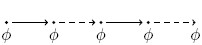
\includegraphics[scale=0.5]{graphics/Ltlalways.png}\\ 
$\diamondsuit \phi$ & $\phi$ has to hold \textbf{eventually} & 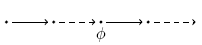
\includegraphics[scale=0.5]{graphics/Ltlevently.png}\\ 
$\bigcirc \phi$ & $\phi$ has to hold \textbf{next} & 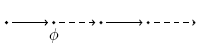
\includegraphics[scale=0.5]{graphics/Ltlnext.png}\\ 
$\psi\U\phi$ & $\psi$ has to hold at least \textbf{until} $\phi$ holds & 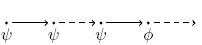
\includegraphics[scale=0.5]{graphics/Ltluntil.png}\\ 
\end{tabular}
\caption{\gls{LTL} quantifiers}
\label{tabl:ltl}
\end{table}


Using \gls{LTL} one can express temporal properties such as 
%
\textit{pointer p is never null}: $\square p (\neq \mbox{null})$ or 
%
\textit{program P finishes}, equivalently, 
%
	program counter reaches the return statement at line $l_k$: $\diamondsuit\pc = l_k$.



\begin{example}
Temporal logic studies problems like the one exposed below.

\label{Collatz:conjecture}

Let $f$ be the following function.

\[
f(n) = \left\{
	\begin{array}{cc}
		\rfrac{n}{2} & \text{ if } (n\text{ mod } 2) \equiv 0\\
		3n+1 & \text{ if } (n\text{ mod } 2) \equiv 1
	\end{array}
\right.
\]

We can form a sequence applying repeatedly $f$. If we take the sequence starting in $n=13$ we get:
%
\[ 
	13 \overset{\displaystyle\;\; 3n+1\;\;}{\longrightarrow}
	40 \overset{\displaystyle\;\;\rfrac{n}{2}\;\;}{\longrightarrow}
	20 \overset{\displaystyle\;\;\rfrac{n}{2}\;\;}{\longrightarrow}
	10 \overset{\displaystyle\;\;\rfrac{n}{2}\;\;}{\longrightarrow}
	5 \overset{\displaystyle\;\; 3n+1\;\;}{\longrightarrow}
	16 \overset{\displaystyle\;\;\rfrac{n}{2}\;\;}{\longrightarrow}
	8 \overset{\displaystyle\;\;\rfrac{n}{2}\;\;}{\longrightarrow}
	4 \overset{\displaystyle\;\;\rfrac{n}{2}\;\;}{\longrightarrow}
	2 \overset{\displaystyle\;\;\rfrac{n}{2}\;\;}{\longrightarrow}
	1
\]
%
One could ask if this sequence eventually stops regardless the integer chosen to begin. This question is called \concept{Collatz conjecture} and has not been solved yet. 
%
For the moment, an infinite sequence has not been found, but the temporal logic problem has not been proven either.
%

We could write in \gls{FOL} the formula for this conjecture as $[ \forall x \exists n (\underbrace{f \circ f \circ  ... \circ f}_{n})(x) = 1]$. However, the temporal formula for this problem is: $\diamondsuit \left(f(n) = 1\right)$
\end{example}


With \gls{LTL} one can express properties a program must hold to work properly. 
%
This properties may be \concept[Safety]{safety properties} or \concept[Liveness]{liveness properties}.


\textbf{Safety properties} are ... \todo{Defn}


\textbf{Liveness properties} are ... \todo{Defn}


\gls{LTL} is a much wider field but just this introduction is needed to talk about formal verification.

